%By tuning ITRDVFS, we achieve a 4x decrease in total time spent on this workload, though that comes at a cost of higher energy consumption rate in Linux tuned.

%This figure also provides context for the interactions that occur between the message size, the protocol stack and the bytes on the wire as message size change. At a large 512 KB message, the network becomes the bottleneck and all three systems start converging at peak throughput, as a larger faction of time is spent on the wire and the system' idle time proportionally increases.  At small to medium sizes more time, per-round trip, is spent in the system code; device driver and protocol processing, thus the load on system's software is proportionally higher.

%At larger message sizes the systems ability to detect and exploit large idle times will be exposed and at small message sizes the systems software's efficiency will be highlighted.  Medium messages sizes will expose a mixture of the systems ability to detect and exploit idle opportunities while also exposing its packet processing efficiency. The less time spent packet processing the greater the opportunity to idle.   

%, thereby illustrating the latency and throughput trade-offs in this application.

%TODO YA
%This figure has the potential to provide context of the different interactions that occur between the workload, protocol stack, and bytes on the wire as message size changes, which illustrates the latency and throughput trade-offs in this application.
%We hypothesize that this result is mainly due to the inefficiencies of the dynamic itr-delay algorithm to adapt to a simple ping-pong workload where a simple static itr-delay value set to a message specific size can result in improved packet processing efficiency. \textbf{as message size changes the workload changes with respective to the protocol stack and bytes on the wire, system tradeoff between latency and throughput changes as size changes}

%% \begin{figure}
%% 	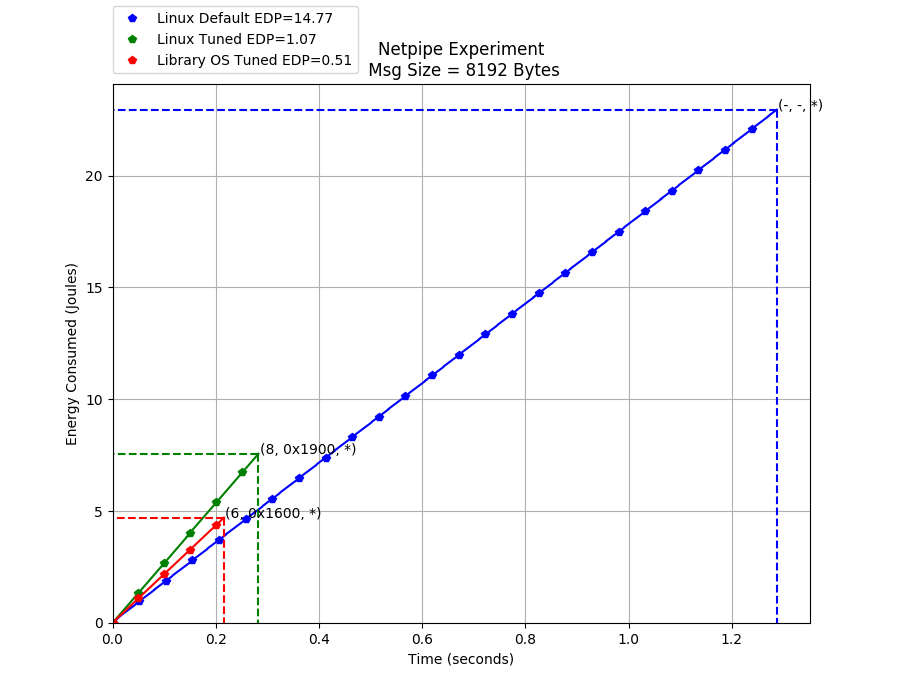
\includegraphics[width=\columnwidth]{asplos2021_figures/netpipe_edp_8192.png}
%% 	\caption{Plot for a fixed message of 8 KB where EDP is minimized.}
%% 	\label{fig:netpipe8192edp}
%% \end{figure}	
%% \begin{figure}
%% 	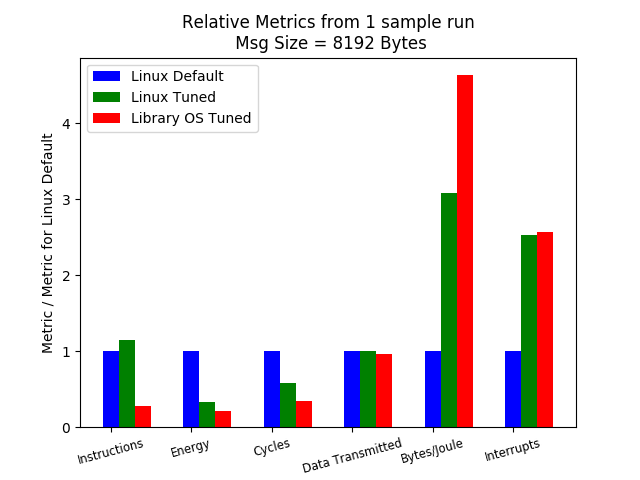
\includegraphics[width=\columnwidth]{asplos2021_figures/netpipe_combined_barplot_8192.png}
%% 	\caption{Raw data collected from logs for 1 sample run of message size 8 KB normalized to Linux default.}
%% 	\label{fig:netpipe8192bar}
%% \end{figure}

\begin{figure}[t]
  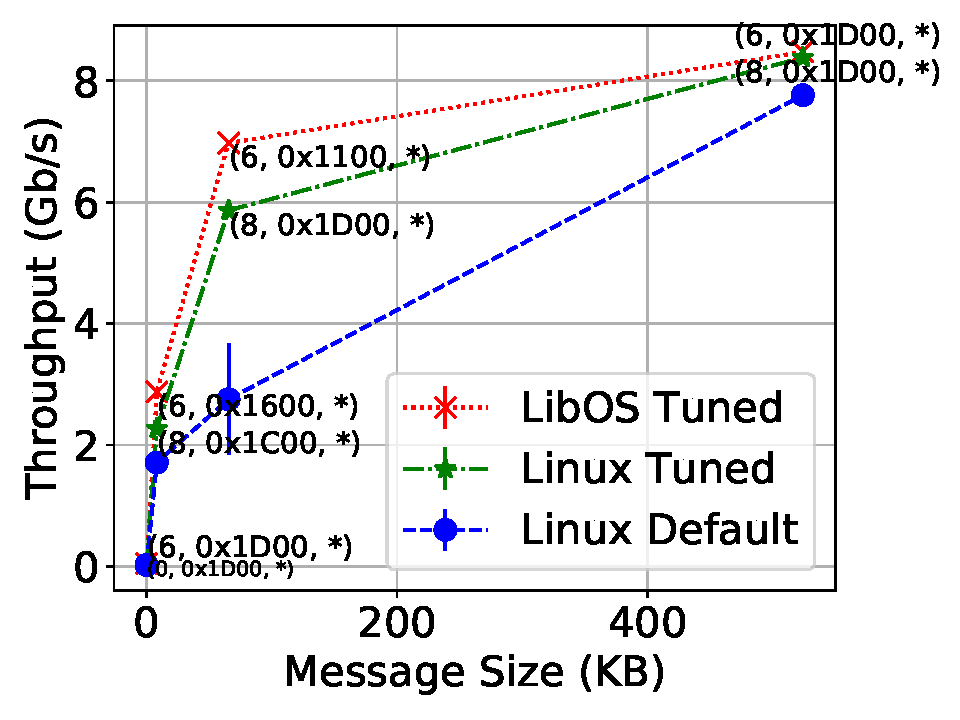
\includegraphics[width=\columnwidth]{osdi_figures/netpipe_tput.pdf}
  \caption{Throughput results across message sizes when tuned for performance.}
  \label{fig:netpipe_tput}
\end{figure}

Figure~\ref{fig:netpipe_tput} illustrates results from a pure throughput perspective across four message sizes (64B up to 512 KB).
By tuning the ITR to a fixed value, we are able to a find a specific hardware configuration for each message size that optimizes overall throughput.
Linux tuned results in a 1.5X to 2X improvement in throughput across message sizes, the libOS further improves the performance by a factor of 1.6X to 3X as compared to Linux. Figure~\ref{fig:netpipe_tput} also shows that as payload size increase, the network becomes the bottleneck and all three systems start converging at peak throughput; this implies that as a larger faction of time is spent on the wire, potentially increasing each systems' idling time. At small to medium payload sizes, there is more of a mix between packet transmission time and time spent in the system code, device driver, and protocol processing.

\subsubsection{General Observations}
From the datapoints listed in Table~\ref{table:eppsum}, Linux tuned outperforms default Linux across all four message sizes in EPP by up to 60\%, further, the LibOS outperforms Linux default across all four message sizes by up to 80\%. We find that in all cases, this is achieved by reducing both time and energy to complete the offered load. We found RAPL to play a minimal role in power tuning for this application given it is not a processor nor memory intensive workload and runs on a single core. In order to observe general trends of hardware tuning effects on Linux and the libOS, we examined the data from a set of low EPP configurations. We found that at smaller message sizes (64 B, 8 KB), ITR plays a pivotal role in reducing EPP given that vast majority of ITR values were less than 10 \micro s, however, there was wide variations in DVFS values for us to make a statement about its usefulness at low message sizes, we suspect the system is largely too lightly loaded for it to play a role. At a message size of 64 KB, the ITR values have largely moved to the 8 - 30 \micro s range, and at 512 KB to the 26 - 38 \micro s range - this is due to packet transmission becoming a larger bottleneck, the larger ITRs used by both Linux tuned and libOS imply a form of artificial packet coalescing is being induced. At these larger message sizes, DVFS plays a more profound role as we see values between \texttt{0xc00 - 0x1500} being consistently applied by Linux tuned and \texttt{0xc00 - 0x1000} being used by the libOS. In addition, the libOS is able to set its DVFS at a value due to its smaller overall codebase, we find that across all message sizes, the instruction usage of libOS is 43\% - 80\% less than Linux and suffered 71\% - 97\% less last-level cache misses. These instruction level efficiences enable the libOS to support the workload while drastically lowering its energy usage through reduced processor frequency; this is also supported by the fact that the libOS's energy usage fell by a greater percentage than time used in the larger message sizes.

\begin{figure}[t]
  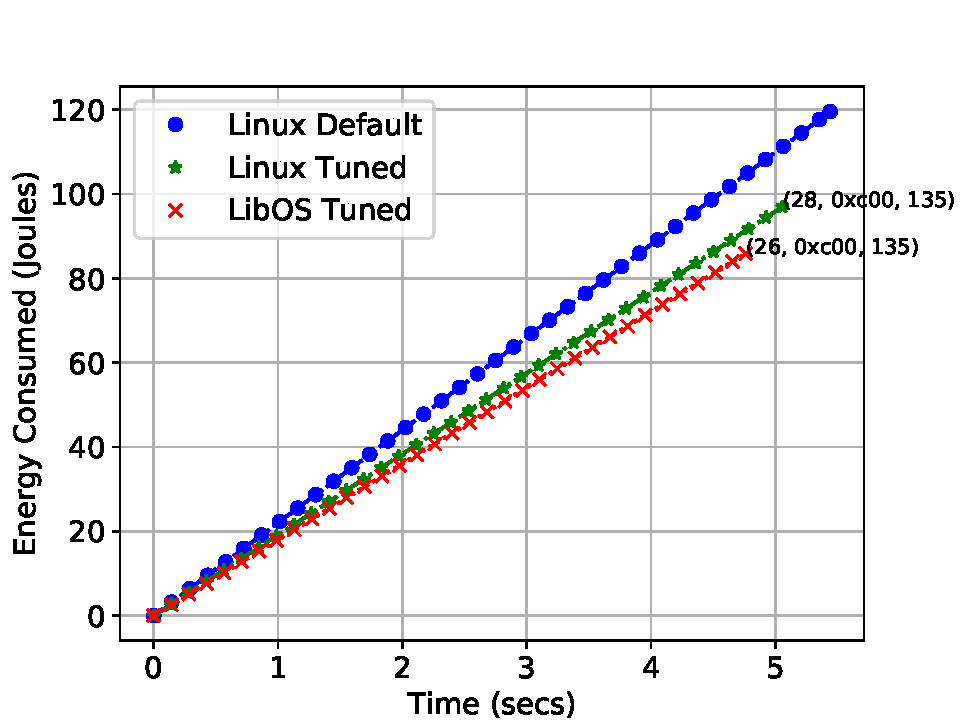
\includegraphics[width=\columnwidth]{osdi_figures/netpipe_524288_epp.pdf}
  \caption{Plot for a fixed message of 512 KB where EPP is minimized.}
  \label{fig:netpipe524288epp}
\end{figure}

\begin{figure*}[htb]
\centering	
\begin{minipage}[t]{0.45\textwidth}
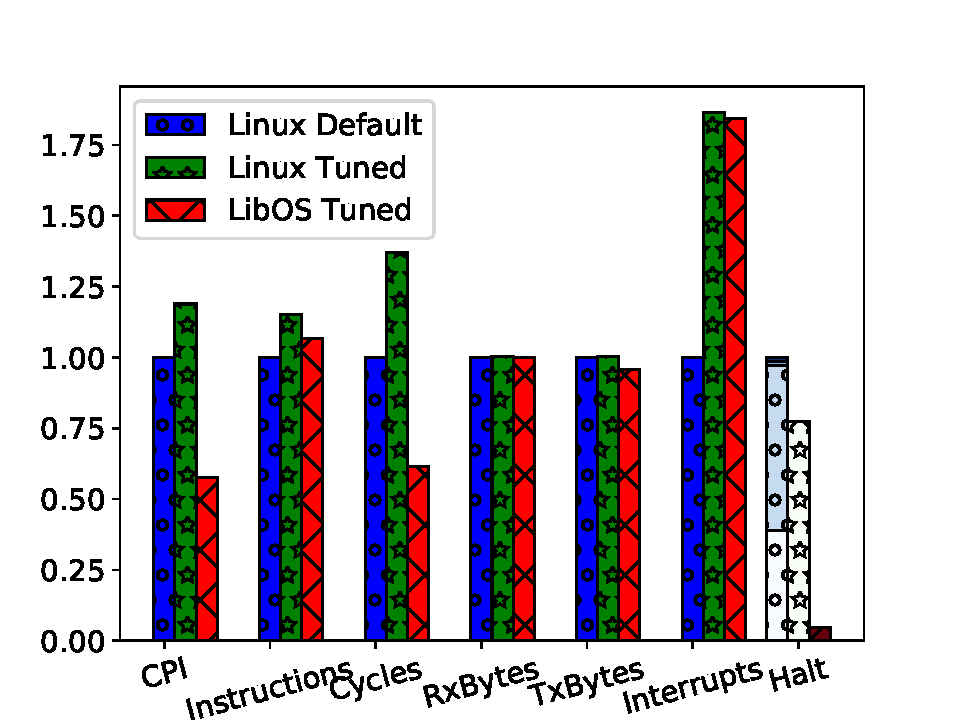
\includegraphics[width=\textwidth]{osdi_figures/netpipe_524288_barplot.pdf}
	\caption{Raw data collected from logs for 1 sample run of message size 512 KB normalized to Linux default.}
	\label{fig:netpipe524288barplot}
\end{minipage}
\begin{minipage}[t]{0.45\textwidth}
	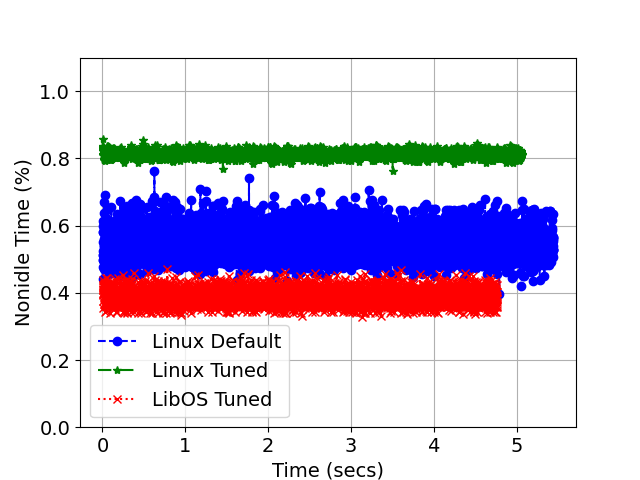
\includegraphics[width=\columnwidth]{osdi_figures/netpipe_524288_nonidle_timeline.png}
	\caption{Per-interrupt non-idle ratio for 512 KB message.}
	\label{fig:netpipe524288nonidle}
\end{minipage}
\begin{minipage}[t]{0.45\textwidth}
	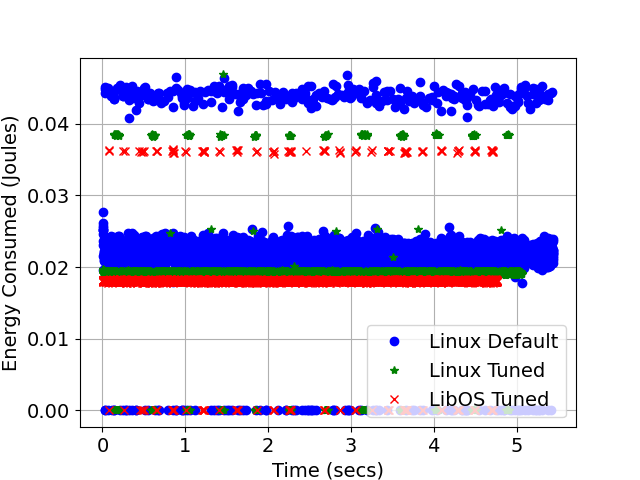
\includegraphics[width=\textwidth]{osdi_figures/netpipe_524288_joule_timeline.png}
	\caption{Per-interrupt joules consumed for 512 KB message.}
	\label{fig:netpipe524288joule}
\end{minipage}
\end{figure*}


\subsubsection{512 KB Analysis}
Figure~\ref{fig:netpipe524288epp} shows the joules consumed as a function of time across the length of the workload that sends fixed-size 512KB messages over 5000 round-trips. The line is generated from the detailed per-interrupt log data, the points illustrated are a sub-sampling to improve legibility.  
The slope in this figure is representative of the rate of energy consumption for each system.
Through hardware tuning, Linux achieves 25\% savings in EPP and the libOS achieves 37\% savings, moreover, the rate of energy consumption has also been lowered.

%Figure~\ref{fig:netpipe8192edp} shows the EDP of running our workloads across the three systems upon tuning the aforementioned hardware knobs  towards lower EDP.

%%This figure shows the joules consumed as a function of time across the length of the workload that sends fixed-size 8KB messages over 5000 netpipe round-trips. The line is generate%%d from the detailed per interrupt log data, the points illustrated are a sub-sampling to improve legibility.
%The slope in this figure is representative of the rate of energy consumption for each system.

%By tuning interrupt-delay and DVFS, we achieve a 4x decrease in total time spent on this workload, though that comes at a cost of higher energy consumption rate in Linux tuned.

Figure~\ref{fig:netpipe524288barplot} shows some collected log data gathered from one sample run of this workload and are all normalized against Linux default. Note, the smaller data transmitted in libOS is due to its simpler TCP/IP stack where there are less options used in its TCP/IP header packets. We observe that while the static tuning of Linux and the libOS both reduced the workload in time and used less energy, the number of interrupts was actually 2X higher than default Linux. We attribute this high number of interrupts to be the statically set ITR delay value of 28 \micro s and 26 \micro s for Linux tuned and libOS respectively. This difference is illustrated in figure~\ref{fig:netpipe524288timediff}, where the time difference between every hardware interrupt is shown as function of time for the entire experiment - this figure shows a much wider range of time between interrupts for default Linux. It also shows that tuned Linux's time between every interrupt is roughly concentrated on the ITR delay value that was set, similar to the libOS, except the libOS also exhibits interrupts with wider differences between them. The implication of these diferences are dependent upon the system.

Figure~\ref{fig:netpipe524288nonidle} shows the percentage of time each system was non-idle every 1 ms (this is due to the sampling period we used in this study for reading PMC registers), the non-idle value is derived by taking the ratio between fixed reference cycle data, which measures un-halted core cycles, and the difference between timestamps. From this figure, we can see distinct behaviors between tuned Linux and the libOS where tuned Linux spent most of its time busy to finish the work fast while the libOS was able to both finish the work fast but also take advantage of idling opportunities. The result of this behavior is shown in figure~\ref{fig:netpipe524288joule}, where the two effects of hardware tuning causes the average energy consumption to be lower than Linux default - the 0 joules in figure~\ref{fig:netpipe524288joule} are due to the fact the joule register can only be sampled at a minimum time interval of 1 ms. The efficiency of the libOS and its ability to idle can be seen in figure~\ref{fig:netpipe524288barplot} where the libOS halted into \texttt{C7} sleep state 3X higher than Linux default and the fact the libOS' CPI is 40\% lower. It is also interesting to note tuning Linux resulted in a completely different behavior in terms of idling state where the tuned Linux concentrated all of its idling in the \texttt{C1} state. We hypothesize this is due to the frequent interrupts invoked by the static ITR delay affecting Linux's scheduler. Moreover, the wide range the libOS' time between interrupts could be explained by the high number of \texttt{C7} sleep states as a \texttt{C7} sleep state has exit latencies in the order of hundreds of microseconds while the \texttt{C1} sleep state's exit latency is 2 \micro s.Moreover, even though Linux tuned could not idle as efficiently as the libOS, both systems could set DVFS to a low value of \texttt{0xc00}. We believe this is due to the network heavy nature of NetPIPE when exchanging 512 KB messages, the benefit of this low DVFS value results in a greater percentage of energy savings than time savings for both tuned Linux and the libOS.

%Compared to default Linux, summing up the total number of times c-state was entered, we found tuned Linux idled 23\% less and the libOS idled 96\% less, however the nature of these sleep states counters do not specify 

%This points to greater aggregate workload efficiency coming from fixed lower interrupt delays, 8 $\micro$s and 6 $\micro$s respectively, than what the default algorithm chooses over the life time of the experiment.   This increase in interrupts in 
%tuning Linux results in a 15\% increase in the overall number of instructions executed, however, the temporal savings this translates to yields a significant improvement in energy used and the energy efficiency of the other metrics.  In some sense tuning allow the systems to race to halt to get the work done by  burning energy at a slightly greater rate but using it more efficiently.  

%In our library OS, the number of instructions per interrupt is lower despite a small increase in total interrupt count due to the smaller interrupt-delay value, it also uses dramatically fewer instruction. This results in a considerably higher Bytes transmitted per joule efficiency. A library OS has shorter path lengths due to its dedicated and simplified processing model, further, as application code is executed in the same privileged domain as the device and protocol code and runs in an integrated fashion with the receive interrupt handler. 


%the energy used to satisfy the same work decreases by 3x.
%This speaks to the instruction efficiency of tuning in relation to improving packet processing time.
%Moreover by tuning a library OS, we are able to both reduce instruction count and energy use while supporting the same workload. 

%% \begin{figure}
%% 	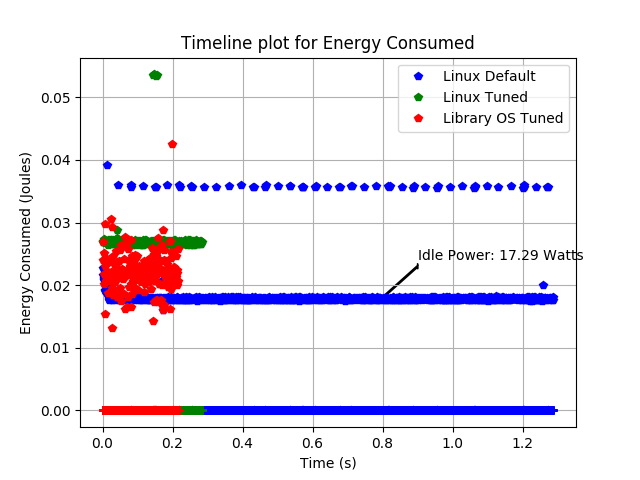
\includegraphics[width=\columnwidth]{asplos2021_figures/netpipe_timeline_joules.png}
%% 	\caption{Per interrupt measure of Joule collected for Netpipe 8KB.}
%% 	\label{fig:netpipe8K_joule_tsc}
%% \end{figure}

%Further packet processing efficiency can be seen in figure~\ref{fig:netpipe8K_joule_tsc}, where the per-interrupt number of joules consumed is shown.
%As joules can only be sampled at a minimum time interval of 1 ms, all three systems will exhibit instances in which the time between interrupts is less than 1 ms.
%This is accounted for in the graph by the bottom band of points that report 0 joule energy consumption. These points effectively visualize the temporal interrupt activity that contributes to the 1ms separated Joule readings.  At the scale plotted, it is a hard to compare the interrupt activity captured by the zero points, however, the interrupt bars of Figure~\ref{fig:netpipe8192bar} can be used to infer the relative difference in density of interrupts along the zero line.

%In default Linux, we see two distinct bands of joules consumed, a sparse band showing higher joule consumption, and a dense middle band showing lower joule consumption.
%A simple back-of-the-envelope calculation summing the joules and dividing by the total time gives us a measure of power at 17.29\watt.  This value is very close to the number we have measured when Linux and our library OS are completely idle, with no user applications launched, and they are able to use the deepest sleep state of the processor for the period that their idle behaviour can halt the processor.  

%It should be noted that an OS idling often involves some component of non-halted, time to conduct various  \textit{idle work} -- maintenance and background system work.  Furthermore,  despite being idle once there is application and network activity an OS may have more "idle work" that it must do and the nature of this work maybe stochastic in its costs (eg. uneven garbage collection work).  Despite halting the processor, the OS may use different and less aggressive sleep states given some algorithm it may have for predicting the value and penalty of the sleep states.  While this is true for Linux which is designed to run many applications over many different scenarios, the library OS we use adopts a simple fixed policy of always halting to the deepest sleep state.  

%With the above in mind, we observe fascinating phenomena when considering Figures~\ref{fig:netpipe8K_joule_tsc} and ~\ref{fig:netpipe8Knonidle}. Figure~\ref{fig:netpipe8Knonidle} is derived by taking the ratio between fixed reference cycle data point, which measures un-halted core cycles, and the measured diff between timestamps. 

%Linux default has a bi-modal behavior where it shows a slow steady rate of work that also idles efficiently (close to the best idle power consumption). Unfortunately this drags the total time well beyond what it could have achieved, in other words it neither raced-to-halt globally nor locally. Moreover, when it is doing work it is also more inefficient compared to Linux and the library OS tuned by using more Joules. However, while Linux tuned also managed to race-to-halt globally per interrupt, it was over 50\% busy, which suggests its algorithms averaging its power consumption between the idle consumption and the busy consumption. In contrast, the library OS's shorter path length and simple idle behaviour allow it to both race to halt globally and between interrupts. Thus the library OS is more effectively exploiting the IO nature of the workload to lower the energy consumption. 
%we observe when default Linux is servicing a packet.  
%This power number is exactly the per-package idle power number that we also measured from past experiments.
%This results tells us that the default Linux policy causes Linux it to spend more time idling (the middle band) than actually doing work (the highest band) and is therefore another contributing factor to its EDP. 

%In tuned Linux, there seems to be no idling time at all due to the use of an extremely fast interrupt-delay of 8 $\micro$s, which suggests the benefit of quick turn-around-time for this particular workload.
%Interestingly, while the library OS uses an even smaller interrupt-delay of 6 $\micro$s, it manages to both respond to packets quickly and take advantage of slack time to idle and conserve more energy.
%Moreover, the library OS's instruction efficiency allows it to tune processor frequency at a lower value than tuned Linux.
%The difference between the library OS's idle efficiency and that of tuned Linux is shown in  figure~\ref{fig:netpipe8Knonidle} which uses data from reference cycles collected.
%Reference cycles count the un-halted core cycles that are not affected by processor frequency tuning.
%Therefore, they can be used to infer potential energy savings from idling by observing its ratio with the timestamp counter.
%NOTE FOR YA
%linux is mostly idling
%linux tuned idles least
%lib os tuned idles more or simply executes less overall

%% \begin{figure}
%% 	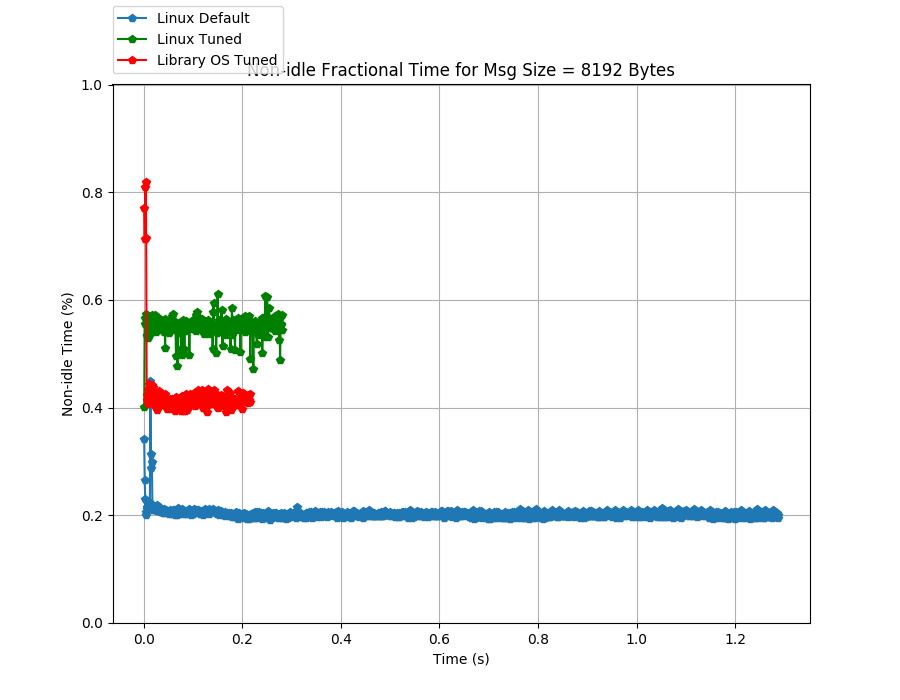
\includegraphics[width=\columnwidth]{asplos2021_figures/netpipe_nonidle_8192.png}
%% 	\caption{Non-idle ratio for fixed message size at 8 KB}
%% 	\label{fig:netpipe8Knonidle}
%% \end{figure}

%Perhaps a potential benefit of the packet transmission behavior a library OS results in the ability to idle at a more efficient rate. In both systems, when there are no packets to be processed the processors are idling and will be put into some sleep state. These sleep states consists of different levels of energy savings by turning off various processor features.  This figure shows that while Linux default spends 20\% of its time processing and therefore 80\% of its time idling, potentially saving energy by going into sleep states, the increased overall processing time means the base idle cost is still a major contributor to overall energy usage. However we find that by using a library OS, it results in middle ground such that the shortened processing time and the simple packet transmission ability of its device driver results more idle time percentage as compared to Linux tuned. 

%\indent \textbf{summarize results from other message sizes}
%While our study includes detailed experiments for the netpipe workloads at other message sizes, however due to space concerns, we choose to focus on the 8K message size for detailed presentation as it allows one to observe a balance in how the systems behave with respect to busy and idle behavior.  With other message sizes the basic trade-offs remain but in different proportions: 1) at 64 byte messages tuning Linux to minimize EDP reduces the time and energy by 25\% and tuning the library OS by yields a 50\% reduction in time and energy compared to Linux default, 2) at 64KB message size 40\% reduction in time and energy for tuned Linux and 60\% for library OS, and at 512 KB message size 5\% and 10\% respectively.
